%! Unidad 1 — Movimiento armónico simple (teoría, actividades resueltas y prácticas)
%! Fuente: Fuentes/Tema1_Movimiento_Armonico_Simple.pdf (reescrito; datos de las actividades cambiados y recalculados)

\section*{Para empezar: el reloj de Huygens}
\addcontentsline{toc}{section}{Para empezar: el reloj de Huygens}

Hasta mediados del siglo \textsc{xvii} los mejores relojes mecánicos podían atrasarse o adelantarse un cuarto de hora al día.
En 1656 Christiaan Huygens construyó el primer reloj de péndulo: aprovechó que un péndulo que oscila con poca amplitud tarda
siempre lo mismo en ir y volver, y el error bajó a menos de un minuto diario. Ese «tardar siempre lo mismo» es la propiedad
central de esta unidad. Los muelles, los péndulos, las cuerdas de una guitarra, los átomos de un sólido o el aire que transmite
un sonido vibran de una forma muy parecida, y todos se describen con el mismo modelo: el \textbf{movimiento armónico simple}.
Además, es la base para estudiar las ondas en las unidades siguientes.

\section{Movimientos periódicos y oscilatorios}\label{sec:mas-periodico}

\begin{definition}[Movimiento periódico]
    Un movimiento es \rojon{periódico} cuando la posición, la velocidad y la aceleración del móvil vuelven a tomar los mismos
    valores a intervalos de tiempo iguales.
\end{definition}

Son periódicos, por ejemplo, el giro de las agujas de un reloj, la rotación de la Tierra o su traslación alrededor del Sol.

Un caso particular son los movimientos de ida y vuelta alrededor de una posición fija. Si separamos un cuerpo de su posición
de equilibrio \(O\) hasta \(A\) y lo soltamos, vuelve hacia \(O\), no se detiene allí, sigue hasta \(B\), se para un instante y
regresa hacia \(A\): \(A \rightarrow O \rightarrow B \rightarrow O \rightarrow A\) (figura~\ref{fig:mas-osciladores}).

\begin{figure}[H]
    \centering
    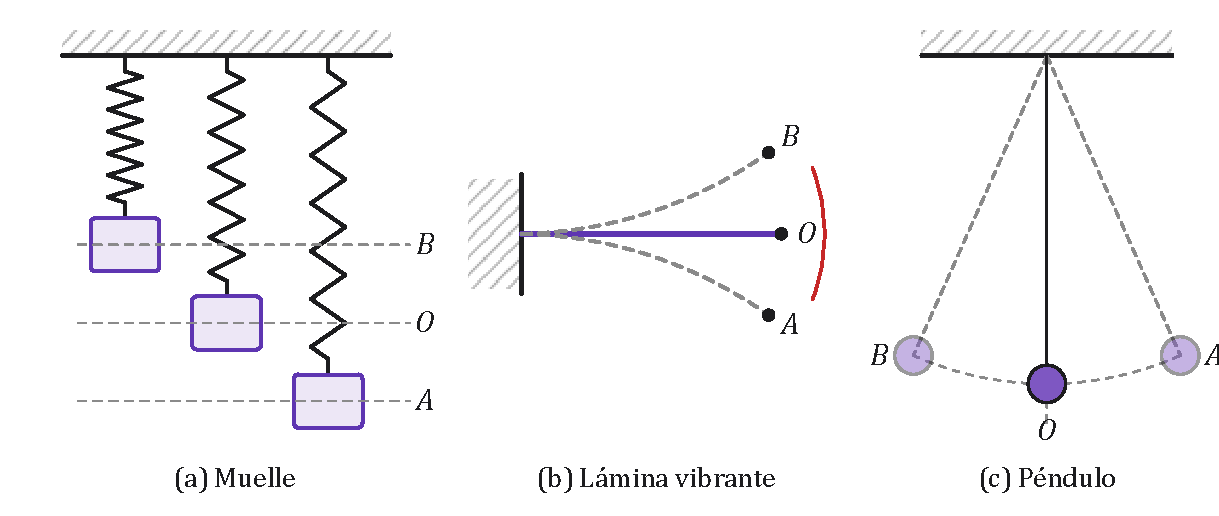
\includegraphics[width=0.9\linewidth]{images/UD1/osciladores}
    \caption{Tres osciladores: una masa colgada de un muelle, una lámina sujeta por un extremo y un péndulo. En los tres
    el cuerpo va y viene entre \(A\) y \(B\) pasando por la posición de equilibrio \(O\).}
    \label{fig:mas-osciladores}
\end{figure}

\begin{definition}[Movimiento oscilatorio]
    Un movimiento periódico es \rojon{oscilatorio} (o vibratorio) cuando el móvil va y viene a uno y otro lado de una posición
    de equilibrio. Cada recorrido completo de ida y vuelta (\(A \rightarrow O \rightarrow B \rightarrow O \rightarrow A\))
    se llama \azuln{oscilación}, \azuln{vibración} o \azuln{ciclo}.
\end{definition}

Para describir la rapidez con que se repite el movimiento se usan dos magnitudes, una inversa de la otra:
\begin{itemize}
    \item \textbf{Período} (\(T\)): tiempo que tarda el móvil en completar una oscilación. Se mide en segundos (\unit{\second}).
    \item \textbf{Frecuencia} (\(\nu\) o \(f\)): número de oscilaciones que realiza en cada unidad de tiempo. Se mide en hercios:
    \(\qty{1}{\hertz} = \qty{1}{\per\second}\) (una oscilación por segundo).
\end{itemize}
\begin{centeredequation}
    T = \dfrac{1}{\nu} \label{eq:mas-T-nu}
\end{centeredequation}

\section{El movimiento armónico simple}\label{sec:mas-definicion}

Entre todos los movimientos oscilatorios hay uno especialmente sencillo y frecuente en la naturaleza.

\begin{definition}[Movimiento armónico simple (m.a.s.)]
    Una partícula describe un \rojon{movimiento armónico simple} cuando oscila sobre un segmento rectilíneo y la fuerza que
    actúa sobre ella es, en cada instante, proporcional a su distancia a la posición de equilibrio y dirigida hacia ella:
    \begin{centeredequation}
        F = -k\,y \label{eq:mas-fuerza}
    \end{centeredequation}
    Esta fuerza se llama \azuln{fuerza recuperadora}. Un cuerpo que se mueve así es un \azuln{oscilador armónico}.
\end{definition}

El signo menos indica que la fuerza siempre apunta en sentido contrario al desplazamiento: si el cuerpo está por encima del
equilibrio (\(y > 0\)) la fuerza tira hacia abajo y si está por debajo (\(y < 0\)), hacia arriba. Como veremos, en un m.a.s. la
posición, la velocidad y la aceleración se expresan con funciones seno y coseno; por eso se llama \emph{armónico}.

\subsection{Magnitudes características}\label{subsec:mas-magnitudes}

\begin{table}[H]
    \centering
    \caption{Magnitudes que describen un movimiento armónico simple}
    \vspace{-5pt}
    \begin{tabular}{@{}lcL{8.2cm}c@{}}
        \toprule
        \textbf{Magnitud} & \textbf{Símbolo} & \textbf{Significado} & \makecell{\textbf{Unidad} \\ \textbf{(SI)}} \\
        \midrule
        Elongación & \(y\) & Posición del móvil medida desde el centro de oscilación (la posición de equilibrio). Puede ser positiva o negativa. & \unit{\m} \\[3pt]
        Amplitud & \(A\) & Valor máximo de la elongación. La distancia entre los dos extremos es \(2A\). & \unit{\m} \\[3pt]
        Período & \(T\) & Tiempo que dura una oscilación completa. & \unit{\second} \\[3pt]
        Frecuencia & \(\nu\) & Número de oscilaciones por segundo: \(\nu = 1/T\). & \unit{\hertz} \\[3pt]
        Pulsación & \(\omega\) & También llamada frecuencia angular: \(\omega = 2\pi/T = 2\pi\nu\). & \unit{\radian\per\second} \\[3pt]
        Fase & \(\omega t + \varphi_0\) & Ángulo que indica el estado de vibración en el instante \(t\). & \unit{\radian} \\[3pt]
        Fase inicial & \(\varphi_0\) & Valor de la fase en \(t = 0\); depende de dónde empieza el movimiento. & \unit{\radian} \\
        \bottomrule
    \end{tabular}
    \label{tab:mas-magnitudes}
\end{table}

\begin{remark}
    La pulsación se mide en \unit{\radian\per\second}, igual que una velocidad angular, pero no es una velocidad angular: en un
    m.a.s. nada gira. Se llama así porque, como veremos enseguida, el m.a.s. se puede obtener proyectando un movimiento circular.
\end{remark}

\section{Cinemática del movimiento armónico simple}\label{sec:mas-cinematica}

\subsection{Ecuación de la posición}\label{subsec:mas-posicion}

La ecuación del m.a.s. da la elongación en función del tiempo, \(y = f(t)\). Para obtenerla usaremos una idea muy útil:

\begin{center}
    \emph{El m.a.s. es la proyección sobre un diámetro de un movimiento circular uniforme.}
\end{center}

Imaginemos un punto \(P\) que recorre una circunferencia de radio \(A\) con velocidad angular constante \(\omega\), y su
sombra sobre el diámetro vertical (figura~\ref{fig:mas-mcu}). Mientras \(P\) da una vuelta, su sombra sube hasta \(+A\),
baja hasta \(-A\) y vuelve al centro: recorre el diámetro dos veces y hace una oscilación completa en el mismo tiempo \(T\)
que tarda \(P\) en dar la vuelta. En un cuarto de vuelta la sombra va del centro a un extremo: recorre la amplitud.

\begin{figure}[H]
    \centering
    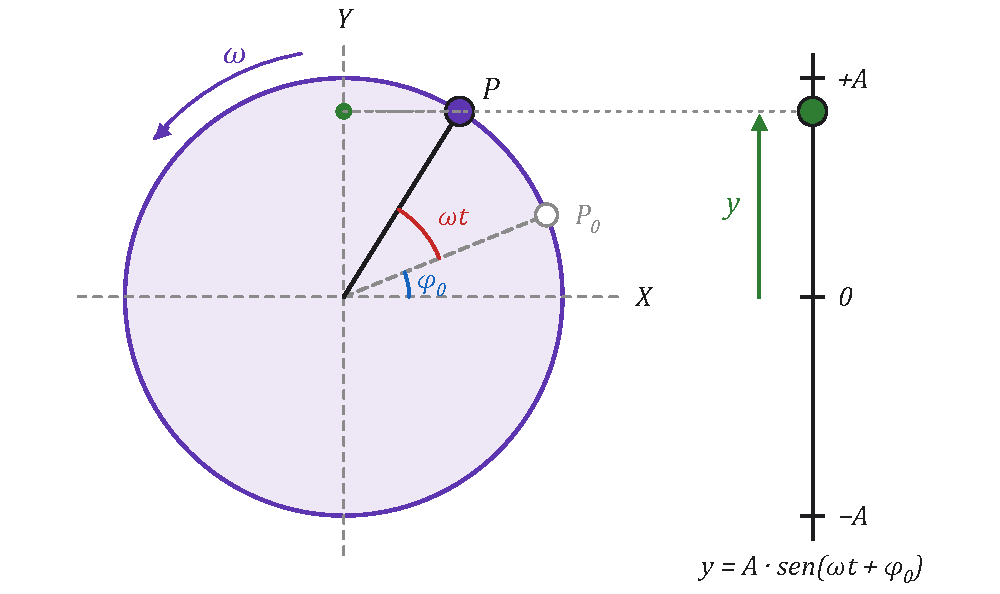
\includegraphics[width=0.72\linewidth]{images/UD1/mas_mcu}
    \caption{El punto \(P\) gira con velocidad angular \(\omega\). Su proyección sobre el diámetro vertical oscila entre
    \(+A\) y \(-A\) con un movimiento armónico simple.}
    \label{fig:mas-mcu}
\end{figure}

Si en \(t = 0\) el punto está en \(P_0\), formando un ángulo \(\varphi_0\) con el eje \(X\), en el instante \(t\) habrá girado
un ángulo \(\omega t\) más. La altura de su proyección es entonces:
\begin{centeredequation}
    \boxed{y = A \sen(\omega t + \varphi_0)} \label{eq:mas-posicion}
\end{centeredequation}

\begin{itemize}
    \item \(A\), \(\omega\) y \(\varphi_0\) son constantes que hay que conocer para escribir la ecuación de un m.a.s. concreto.
    \item \(\omega t + \varphi_0\) es la \azuln{fase}: determina el estado de vibración (posición y sentido del movimiento) en cada instante.
    \item \(\varphi_0\) es la \azuln{fase inicial}. Se calcula con las condiciones iniciales, es decir, con la posición (y el
    sentido del movimiento) en \(t = 0\).
\end{itemize}

Si proyectamos sobre el eje horizontal se obtiene \(x = A\cos(\omega t + \varphi_0)\). Ambas formas son equivalentes (solo
cambia el valor de \(\varphi_0\), porque \(\cos\alpha = \sen(\alpha + \pi/2)\)); en este libro usaremos la del seno.

\begin{remark}
    En las ecuaciones del m.a.s. los ángulos están en radianes: \textbf{hay que poner la calculadora en modo RAD}.
\end{remark}

\paragraph{Puntos en fase y en oposición de fase.} La diferencia de fase entre dos instantes \(t_1\) y \(t_2\) del mismo
movimiento es:
\begin{equation*}
    \Delta\varphi = (\omega t_2 + \varphi_0) - (\omega t_1 + \varphi_0) = \omega\,(t_2 - t_1) = \omega\,\Delta t
\end{equation*}
\begin{itemize}
    \item Están \rojon{en fase} si \(\Delta\varphi = 2n\pi\) (\(n = 1, 2, 3\ldots\)): el móvil está en la misma posición y se
    mueve en el mismo sentido. Ocurre cuando \(\Delta t = nT\).
    \item Están \rojon{en oposición de fase} si \(\Delta\varphi = (2n-1)\pi\): las elongaciones son opuestas y el móvil se
    mueve en sentidos contrarios.
\end{itemize}

\begin{exercise}
    ¿Qué intervalo de tiempo separa dos instantes en los que un m.a.s. está en oposición de fase?
    \begin{solu}
        \textcolor{blue}{En oposición de fase \(\Delta\varphi = (2n-1)\pi\). Como \(\Delta\varphi = \omega\,\Delta t = \dfrac{2\pi}{T}\,\Delta t\):}
        \[ \dfrac{2\pi}{T}\,\Delta t = (2n-1)\pi \quad\Rightarrow\quad \textcolor{red}{\Delta t = (2n-1)\,\dfrac{T}{2}} \]
        \textcolor{red}{Un número impar de medios períodos: \(T/2\), \(3T/2\), \(5T/2\ldots\)}
    \end{solu}
\end{exercise}

\begin{exercise}
    Un cuerpo colgado de un muelle oscila con un m.a.s. de \qty{12}{\cm} de amplitud y \qty{0.2}{\second} de período. En
    \(t = 0\) el muelle está en su máximo alargamiento, que tomamos como elongación negativa. Escribe la ecuación del movimiento.
    \begin{solu}
        \textcolor{blue}{Ecuación general: \(y = A\sen(\omega t + \varphi_0)\), con \(A = \qty{0.12}{\m}\).}

        \textcolor{blue}{Pulsación: \(\omega = \dfrac{2\pi}{T} = \dfrac{2\pi}{0{,}2} = 10\pi\ \unit{\radian\per\second}\).}

        \textcolor{blue}{Fase inicial: en \(t = 0\), \(y = -A\): \(-0{,}12 = 0{,}12 \sen\varphi_0 \Rightarrow \sen\varphi_0 = -1
        \Rightarrow \varphi_0 = \dfrac{3\pi}{2}\ \unit{\radian}\).}
        \[ \textcolor{red}{y = 0{,}12\,\sen\!\left(10\pi t + \dfrac{3\pi}{2}\right)\ \text{(m)}} \]
    \end{solu}
\end{exercise}

\begin{exercise}
    Una partícula con m.a.s. sale del extremo positivo de su trayectoria y tarda \qty{0.5}{\second} en llegar al centro, que
    está a \qty{15}{\cm}. Calcula:
    \begin{enumerate}[label=\letraminuscula]
        \item La frecuencia.
        \item La ecuación del movimiento.
        \item La posición \qty{1}{\second} después de empezar.
    \end{enumerate}
    \begin{solu}
        \textcolor{blue}{Del extremo al centro hay un cuarto de oscilación: \(T/4 = \qty{0.5}{\second} \Rightarrow T = \qty{2}{\second}\);
        y la distancia es la amplitud: \(A = \qty{0.15}{\m}\).}
        \begin{enumerate}[label=\letraminuscula]
            \item \(\nu = \dfrac{1}{T} = \textcolor{red}{\qty{0.5}{\hertz}}\).
            \item \textcolor{blue}{\(\omega = 2\pi/T = \pi\ \unit{\radian\per\second}\). En \(t = 0\), \(y = A\): \(\sen\varphi_0 = 1 \Rightarrow \varphi_0 = \pi/2\).}
            \(\textcolor{red}{y = 0{,}15\,\sen\!\left(\pi t + \dfrac{\pi}{2}\right)\ \text{(m)}}\)
            \item \(y(1) = 0{,}15\,\sen\!\left(\pi + \dfrac{\pi}{2}\right) = 0{,}15\cdot(-1) = \textcolor{red}{\qty{-0.15}{\m}}\):
            al cabo de medio período está en el otro extremo.
        \end{enumerate}
    \end{solu}
\end{exercise}

\begin{exercise}
    Una partícula con m.a.s. recorre un segmento de \qty{10}{\cm} (de un extremo al otro) en \qty{0.04}{\second}. En \(t = 0\)
    su elongación es máxima y positiva. Calcula:
    \begin{enumerate}[label=\letraminuscula]
        \item La ecuación del movimiento.
        \item La posición en \(t = \qty{1.3}{\second}\).
        \item La diferencia de fase entre ese instante y el inicial.
    \end{enumerate}
    \begin{solu}
        \textcolor{blue}{Datos: \(2A = \qty{10}{\cm} \Rightarrow A = \qty{0.05}{\m}\). Ir de un extremo al otro es media
        oscilación: \(T/2 = \qty{0.04}{\second} \Rightarrow T = \qty{0.08}{\second}\).}
        \begin{enumerate}[label=\letraminuscula]
            \item \textcolor{blue}{\(\omega = \dfrac{2\pi}{0{,}08} = 25\pi\ \unit{\radian\per\second}\); con \(y(0) = A\), \(\varphi_0 = \pi/2\).}
            \(\textcolor{red}{y = 0{,}05\,\sen\!\left(25\pi t + \dfrac{\pi}{2}\right)\ \text{(m)}}\)
            \item \(y(1{,}3) = 0{,}05\,\sen(32{,}5\pi + 0{,}5\pi) = 0{,}05\,\sen(33\pi) = \textcolor{red}{0}\): pasa por el centro.
            \item \(\Delta\varphi = \omega\,\Delta t = 25\pi\cdot 1{,}3 = \textcolor{red}{32{,}5\pi\ \unit{\radian}}\).
        \end{enumerate}
    \end{solu}
\end{exercise}

\subsection{Ecuación de la velocidad}\label{subsec:mas-velocidad}

La velocidad es la derivada de la posición respecto del tiempo:
\begin{centeredequation}
    \boxed{v = \dfrac{dy}{dt} = A\,\omega\cos(\omega t + \varphi_0)} \label{eq:mas-velocidad}
\end{centeredequation}

Usando \(\sen^2\alpha + \cos^2\alpha = 1\) podemos expresarla en función de la posición:
\begin{equation*}
    v = \pm A\omega\sqrt{1 - \sen^2(\omega t + \varphi_0)} = \pm\,\omega\sqrt{A^2 - A^2\sen^2(\omega t + \varphi_0)}
    \quad\Rightarrow\quad \boxed{v = \pm\,\omega\sqrt{A^2 - y^2}}
\end{equation*}
El signo depende del sentido en que se mueve el cuerpo. La velocidad:
\begin{itemize}
    \item es \textbf{máxima} en el centro (\(y = 0\)): \(v_{\text{máx}} = A\,\omega\);
    \item es \textbf{nula} en los extremos (\(y = \pm A\)), donde el cuerpo se para para cambiar de sentido.
\end{itemize}

\begin{exercise}
    Un m.a.s. tiene por ecuación \(y = 0{,}3\,\sen(4\pi t + \pi)\) (SI). Calcula:
    \begin{enumerate}[label=\letraminuscula]
        \item La amplitud, la pulsación, el período, la frecuencia y la fase inicial.
        \item La velocidad en \(t = 0\), la velocidad máxima y la velocidad en \(t = \qty{0.5}{\second}\).
    \end{enumerate}
    \begin{solu}
        \begin{enumerate}[label=\letraminuscula]
            \item \textcolor{blue}{Comparando con \(y = A\sen(\omega t + \varphi_0)\):}
            \textcolor{red}{\(A = \qty{0.3}{\m}\); \(\omega = 4\pi\ \unit{\radian\per\second}\); \(T = \dfrac{2\pi}{4\pi} = \qty{0.5}{\second}\);
            \(\nu = \qty{2}{\hertz}\); \(\varphi_0 = \pi\ \unit{\radian}\).}
            \item \textcolor{blue}{\(v = A\omega\cos(\omega t + \varphi_0) = 1{,}2\pi\cos(4\pi t + \pi)\).}
            \begin{itemize}
                \item \(v(0) = 1{,}2\pi\cos\pi = \textcolor{red}{-1{,}2\pi \approx \qty{-3.77}{\m\per\second}}\).
                \item \(v_{\text{máx}} = A\omega = \textcolor{red}{1{,}2\pi \approx \qty{3.77}{\m\per\second}}\).
                \item \(v(0{,}5) = 1{,}2\pi\cos(3\pi) = \textcolor{red}{\qty{-3.77}{\m\per\second}}\) (ha pasado un período: igual que en \(t = 0\)).
            \end{itemize}
        \end{enumerate}
    \end{solu}
\end{exercise}

\subsection{Ecuación de la aceleración}\label{subsec:mas-aceleracion}

Derivando la velocidad:
\begin{centeredequation}
    \boxed{a = \dfrac{dv}{dt} = -A\,\omega^2\sen(\omega t + \varphi_0) = -\,\omega^2\,y} \label{eq:mas-aceleracion}
\end{centeredequation}

La ecuación \(a = -\omega^2 y\) es la «huella» de un m.a.s.: la aceleración es proporcional a la elongación y de signo
contrario. Por tanto:
\begin{itemize}
    \item es \textbf{nula} en el centro y \textbf{máxima} en los extremos: \(a_{\text{máx}} = A\,\omega^2\);
    \item siempre apunta hacia la posición de equilibrio;
    \item está desfasada \(\pi/2\) respecto de la velocidad y \(\pi\) respecto de la posición.
\end{itemize}

\begin{exercise}
    Un móvil con m.a.s. recorre un segmento de \qty{6}{\cm}. Su frecuencia es \qty{5}{\hertz} y en \(t = 0\) pasa por la
    posición de equilibrio moviéndose en sentido positivo. Calcula:
    \begin{enumerate}[label=\letraminuscula]
        \item La ecuación del movimiento.
        \item La velocidad y la aceleración en \(t = 0\).
    \end{enumerate}
    \begin{solu}
        \textcolor{blue}{\(A = \qty{0.03}{\m}\); \(\omega = 2\pi\nu = 10\pi\ \unit{\radian\per\second}\).}
        \begin{enumerate}[label=\letraminuscula]
            \item \textcolor{blue}{En \(t = 0\), \(y = 0\) y \(v > 0\): \(\sen\varphi_0 = 0\) con \(\cos\varphi_0 > 0 \Rightarrow \varphi_0 = 0\).}
            \(\textcolor{red}{y = 0{,}03\,\sen(10\pi t)\ \text{(m)}}\)
            \item \(v(0) = A\omega\cos 0 = 0{,}03\cdot 10\pi = \textcolor{red}{0{,}3\pi \approx \qty{0.94}{\m\per\second}}\) (la máxima);
            \(a(0) = -\omega^2\cdot 0 = \textcolor{red}{0}\).
        \end{enumerate}
    \end{solu}
\end{exercise}

\begin{exercise}
    Una partícula vibra con una amplitud de \qty{5}{\cm} y su velocidad máxima es \qty{15}{\m\per\second}. Calcula:
    \begin{enumerate}[label=\letraminuscula]
        \item La frecuencia del movimiento.
        \item La aceleración máxima.
    \end{enumerate}
    \begin{solu}
        \begin{enumerate}[label=\letraminuscula]
            \item \textcolor{blue}{\(v_{\text{máx}} = A\omega \Rightarrow \omega = \dfrac{15}{0{,}05} = \qty{300}{\radian\per\second}\);}
            \(\nu = \dfrac{\omega}{2\pi} = \textcolor{red}{\qty{47.7}{\hertz}}\).
            \item \(a_{\text{máx}} = A\omega^2 = 0{,}05\cdot 300^2 = \textcolor{red}{\qty{4500}{\m\per\second\squared}}\).
        \end{enumerate}
    \end{solu}
\end{exercise}

\subsection{Representaciones gráficas}\label{subsec:mas-graficas}

Tomemos \(\varphi_0 = 0\): \(y = A\sen\omega t\), \(v = A\omega\cos\omega t\) y \(a = -A\omega^2\sen\omega t\). Calculando
los valores a lo largo de un período (tabla~\ref{tab:mas-valores}) obtenemos las gráficas de la figura~\ref{fig:mas-graficas}.

\begin{table}[H]
    \centering
    \caption{Posición, velocidad y aceleración a lo largo de un período (\(\varphi_0 = 0\))}
    \vspace{-5pt}
    \begin{tabular}{@{}ccccc@{}}
        \toprule
        \(t\) & \(\omega t\) (\unit{\radian}) & \(y\) & \(v\) & \(a\) \\
        \midrule
        \(0\) & \(0\) & \(0\) & \(A\omega\) & \(0\) \\[3pt]
        \(T/4\) & \(\pi/2\) & \(A\) & \(0\) & \(-A\omega^2\) \\[3pt]
        \(T/2\) & \(\pi\) & \(0\) & \(-A\omega\) & \(0\) \\[3pt]
        \(3T/4\) & \(3\pi/2\) & \(-A\) & \(0\) & \(A\omega^2\) \\[3pt]
        \(T\) & \(2\pi\) & \(0\) & \(A\omega\) & \(0\) \\
        \bottomrule
    \end{tabular}
    \label{tab:mas-valores}
\end{table}

\begin{figure}[H]
    \centering
    \begin{tikzpicture}
        \begin{axis}[fisica, xmin=0, xmax=1.12, ymin=-1.3, ymax=1.35, xlabel={\(t\)}, ylabel={\(y\)},
            xtick={0.25,0.5,0.75,1}, xticklabels={\(\frac{T}{4}\),\(\frac{T}{2}\),\(\frac{3T}{4}\),\(T\)},
            ytick={-1,1}, yticklabels={\(-A\),\(A\)}]
            \addplot[domain=0:1, very thick, ocre] {sin(deg(2*pi*x))};
        \end{axis}
    \end{tikzpicture}\hfill
    \begin{tikzpicture}
        \begin{axis}[fisica, xmin=0, xmax=1.12, ymin=-1.3, ymax=1.35, xlabel={\(t\)}, ylabel={\(v\)},
            xtick={0.25,0.5,0.75,1}, xticklabels={\(\frac{T}{4}\),\(\frac{T}{2}\),\(\frac{3T}{4}\),\(T\)},
            ytick={-1,1}, yticklabels={\(-A\omega\),\(A\omega\)}]
            \addplot[domain=0:1, very thick, blue] {cos(deg(2*pi*x))};
        \end{axis}
    \end{tikzpicture}\hfill
    \begin{tikzpicture}
        \begin{axis}[fisica, xmin=0, xmax=1.12, ymin=-1.3, ymax=1.35, xlabel={\(t\)}, ylabel={\(a\)},
            xtick={0.25,0.5,0.75,1}, xticklabels={\(\frac{T}{4}\),\(\frac{T}{2}\),\(\frac{3T}{4}\),\(T\)},
            ytick={-1,1}, yticklabels={\(-A\omega^2\),\(A\omega^2\)}]
            \addplot[domain=0:1, very thick, red] {-sin(deg(2*pi*x))};
        \end{axis}
    \end{tikzpicture}
    \caption{Elongación, velocidad y aceleración de un m.a.s. con \(\varphi_0 = 0\). La velocidad va un cuarto de período
    adelantada respecto de la posición y la aceleración está en oposición de fase con la posición.}
    \label{fig:mas-graficas}
\end{figure}

\section{Dinámica del movimiento armónico simple}\label{sec:mas-dinamica}

\subsection{Ley de Hooke y constante elástica}\label{subsec:mas-hooke}

Si colgamos un cuerpo de masa \(m\) de un muelle de masa despreciable y longitud natural \(l_0\), el muelle se estira hasta
una longitud \(l\) y el cuerpo queda en reposo (figura~\ref{fig:mas-hooke}). El \azuln{alargamiento} es \(\Delta l = l - l_0\).

\begin{figure}[H]
    \centering
    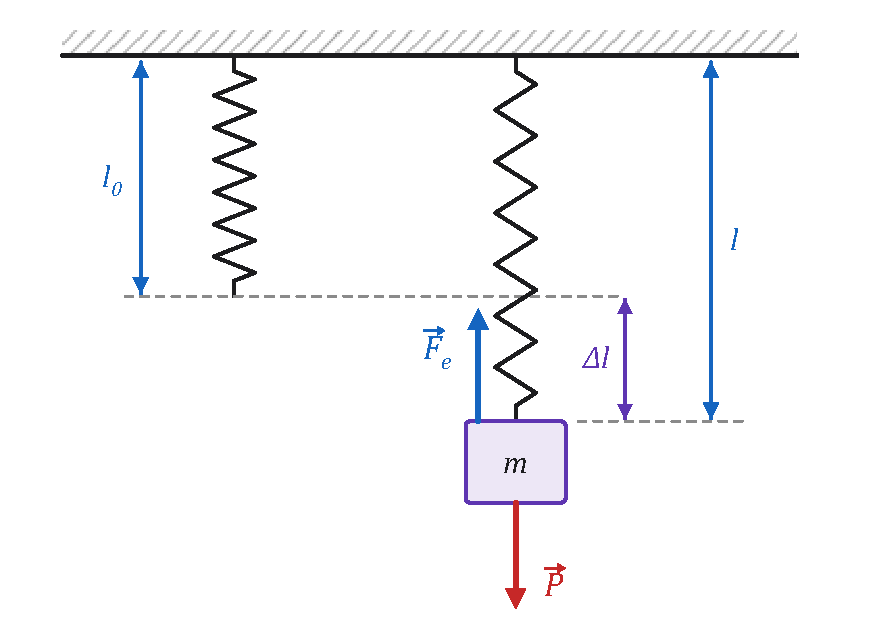
\includegraphics[width=0.55\linewidth]{images/UD1/muelle_hooke}
    \caption{Al colgar la masa, el muelle se alarga \(\Delta l\) hasta que la fuerza elástica equilibra al peso.}
    \label{fig:mas-hooke}
\end{figure}

Sobre el cuerpo actúan su peso y la fuerza elástica del muelle, que según la \rojon{ley de Hooke} es proporcional al
alargamiento, \(F_e = k\,\Delta l\). En el equilibrio:
\begin{equation*}
    \sum\vec F = 0 \;\Rightarrow\; P = F_e \;\Rightarrow\; m g = k\,(l - l_0) \;\Rightarrow\; \boxed{k = \dfrac{m g}{\Delta l}}
\end{equation*}
\(k\) es la \azuln{constante elástica} del muelle y se mide en \unit{\newton\per\m}: cuanto mayor es, más «duro» es el muelle.

\subsection{La fuerza recuperadora}\label{subsec:mas-recuperadora}

Si separamos el cuerpo de su posición de equilibrio y lo soltamos, el muelle ejerce una fuerza neta que tiende a devolverlo a
ella. Lo vemos más claro con un muelle horizontal sin rozamiento (figura~\ref{fig:mas-horizontal}):
\begin{itemize}
    \item si el cuerpo está a la derecha del equilibrio (\(x > 0\)), el muelle tira hacia la izquierda;
    \item si está a la izquierda (\(x < 0\)), lo empuja hacia la derecha;
    \item en la posición de equilibrio (\(x = 0\)) la fuerza es nula.
\end{itemize}

\begin{figure}[H]
    \centering
    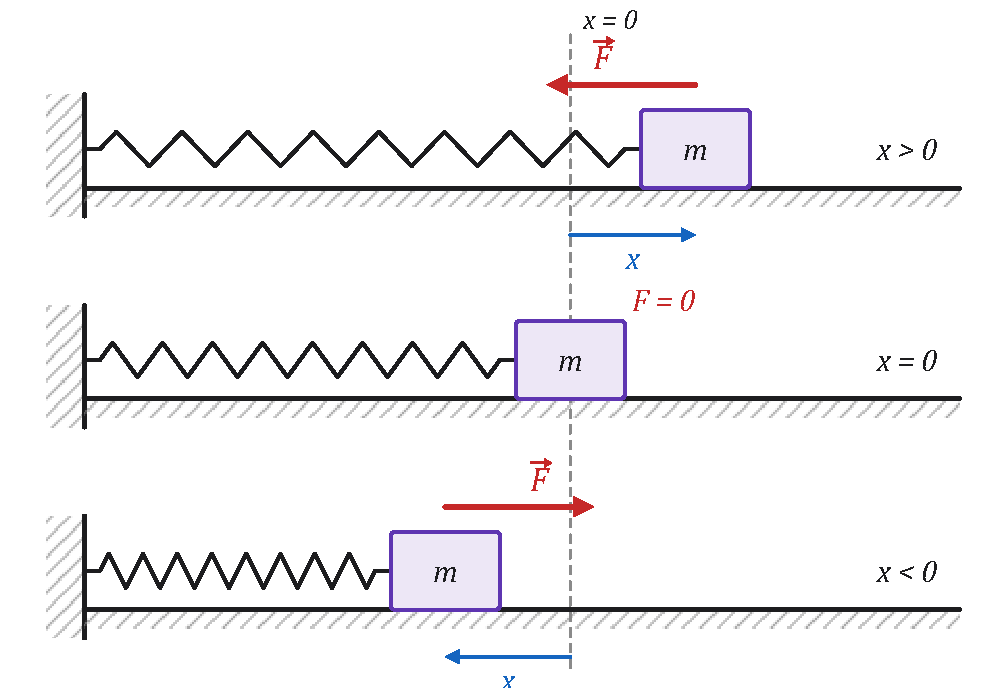
\includegraphics[width=0.72\linewidth]{images/UD1/muelle_horizontal}
    \caption{La fuerza del muelle es siempre opuesta al desplazamiento \(x\) respecto del equilibrio: \(F = -k\,x\).}
    \label{fig:mas-horizontal}
\end{figure}

Es exactamente la fuerza de la ecuación~\eqref{eq:mas-fuerza}, \(F = -k\,y\) (llamaremos \(y\) o \(x\) a la elongación según
la dirección del movimiento). En un muelle vertical ocurre lo mismo si medimos \(y\) desde la nueva posición de equilibrio
con la masa colgada: el peso queda compensado y la fuerza neta vuelve a ser \(-k\,y\).

Aplicando la segunda ley de Newton con la aceleración del m.a.s., \(a = -\omega^2 y\):
\begin{equation*}
    F = m\,a \;\Rightarrow\; -k\,y = -m\,\omega^2\,y \;\Rightarrow\; \boxed{k = m\,\omega^2}
\end{equation*}
y como \(\omega = 2\pi/T\):
\begin{centeredequation}
    \omega = \sqrt{\dfrac{k}{m}} \qquad\qquad \boxed{T = 2\pi\sqrt{\dfrac{m}{k}}} \label{eq:mas-periodo-muelle}
\end{centeredequation}

\begin{remark}
    El período de un oscilador depende solo de la masa y de la constante elástica, \textbf{no de la amplitud}: si lo
    separamos más, recorre más camino pero también va más deprisa, y tarda lo mismo. En los extremos la fuerza es máxima,
    \(F_{\text{máx}} = k\,A\).
\end{remark}

\begin{exercise}
    Si se triplica la masa que cuelga de un muelle, ¿cómo cambia la frecuencia de oscilación?
    \begin{solu}
        \textcolor{blue}{\(\nu = \dfrac{1}{T} = \dfrac{1}{2\pi}\sqrt{\dfrac{k}{m}}\). Con el mismo muelle (\(k\) igual):}
        \[ \dfrac{\nu_2}{\nu_1} = \sqrt{\dfrac{m_1}{m_2}} = \sqrt{\dfrac{m_1}{3m_1}} = \dfrac{1}{\sqrt 3} \;\Rightarrow\; \textcolor{red}{\nu_2 \approx 0{,}58\,\nu_1} \]
        \textcolor{red}{La frecuencia se divide por \(\sqrt 3\) (el muelle oscila más despacio).}
    \end{solu}
\end{exercise}

\begin{exercise}
    Un muelle mide \qty{30}{\cm} cuando cuelga de él una masa de \qty{200}{\g}. Si se añaden \qty{300}{\g} más, mide
    \qty{36}{\cm}. Calcula la constante elástica y la longitud del muelle sin carga.
    \begin{solu}
        \textcolor{blue}{La masa añadida (\qty{0.3}{\kg}) produce un alargamiento adicional de \qty{0.06}{\m}:}
        \[ k = \dfrac{\Delta m\,g}{\Delta l} = \dfrac{0{,}3\cdot 9{,}8}{0{,}06} = \textcolor{red}{\qty{49}{\newton\per\m}} \]
        \textcolor{blue}{Con \qty{0.2}{\kg}: \(0{,}2\cdot 9{,}8 = 49\,(0{,}30 - l_0) \Rightarrow 0{,}30 - l_0 = 0{,}04\)}
        \(\Rightarrow \textcolor{red}{l_0 = \qty{0.26}{\m} = \qty{26}{\cm}}\).
    \end{solu}
\end{exercise}

\begin{exercise}
    Un muelle se alarga \qty{5}{\cm} cuando se cuelga de él un cuerpo de \qty{10}{\kg}. Después se estira \qty{2}{\cm} más
    hacia abajo y se suelta. Tomando como positivo el sentido hacia arriba:
    \begin{enumerate}[label=\letraminuscula]
        \item Calcula la pulsación y el período.
        \item Escribe la ecuación del movimiento.
        \item Calcula la elongación, la velocidad, la aceleración y la fuerza recuperadora en \(t = \qty{1.5}{\second}\).
    \end{enumerate}
    \begin{solu}
        \begin{enumerate}[label=\letraminuscula]
            \item \textcolor{blue}{\(k = \dfrac{mg}{\Delta l} = \dfrac{10\cdot 9{,}8}{0{,}05} = \qty{1960}{\newton\per\m}\);}
            \(\omega = \sqrt{\dfrac{k}{m}} = \sqrt{196} = \textcolor{red}{\qty{14}{\radian\per\second}}\);
            \(T = \dfrac{2\pi}{\omega} = \textcolor{red}{\qty{0.449}{\second}}\).
            \item \textcolor{blue}{\(A = \qty{0.02}{\m}\) y en \(t = 0\) está en \(y = -A\): \(\sen\varphi_0 = -1 \Rightarrow \varphi_0 = 3\pi/2\).}
            \(\textcolor{red}{y = 0{,}02\,\sen\!\left(14 t + \dfrac{3\pi}{2}\right)\ \text{(m)}}\)
            \item \textcolor{blue}{En \(t = \qty{1.5}{\second}\) la fase vale \(14\cdot 1{,}5 + 3\pi/2 = \qty{25.71}{\radian}\) (calculadora en RAD):}
            \begin{itemize}
                \item \(y = 0{,}02\,\sen(25{,}71) = \textcolor{red}{\qty{1.10e-2}{\m}}\)
                \item \(v = 0{,}02\cdot 14\cos(25{,}71) = \textcolor{red}{\qty{0.234}{\m\per\second}}\)
                \item \(a = -\omega^2 y = -196\cdot 1{,}10\cdot 10^{-2} = \textcolor{red}{\qty{-2.15}{\m\per\second\squared}}\)
                \item \(F = -k\,y = -1960\cdot 1{,}10\cdot 10^{-2} = \textcolor{red}{\qty{-21.5}{\newton}}\)
            \end{itemize}
        \end{enumerate}
    \end{solu}
\end{exercise}

\begin{exercise}
    Un muelle de constante \qty{40}{\newton\per\m} mide \qty{25}{\cm} cuando cuelga de él una masa de \qty{0.4}{\kg}.
    \begin{enumerate}[label=\letraminuscula]
        \item ¿Cuánto mide sin carga?
        \item ¿Cuánto medirá si a la masa anterior se le añade otra de \qty{1.5}{\kg}?
    \end{enumerate}
    \begin{solu}
        \begin{enumerate}[label=\letraminuscula]
            \item \(\Delta l = \dfrac{mg}{k} = \dfrac{0{,}4\cdot 9{,}8}{40} = \qty{0.098}{\m}\);
            \(l_0 = 0{,}25 - 0{,}098 = \textcolor{red}{\qty{0.152}{\m} = \qty{15.2}{\cm}}\).
            \item \(\Delta l = \dfrac{1{,}9\cdot 9{,}8}{40} = \qty{0.466}{\m}\);
            \(l = 0{,}152 + 0{,}466 = \textcolor{red}{\qty{0.618}{\m} = \qty{61.8}{\cm}}\).
        \end{enumerate}
    \end{solu}
\end{exercise}

\section{El péndulo simple}\label{sec:mas-pendulo}

Un \rojon{péndulo simple} es una masa pequeña colgada de un hilo inextensible y de masa despreciable. En reposo, el peso y la
tensión del hilo se equilibran (\(\vec P + \vec T = 0\)). Si lo separamos un ángulo \(\varphi\), el peso se descompone en dos
partes (figura~\ref{fig:mas-pendulo}):
\begin{itemize}
    \item \(m g\cos\varphi\), en la dirección del hilo, que queda compensada por la tensión;
    \item \(m g\sen\varphi\), tangente a la trayectoria, que es la que mueve el péndulo hacia la posición de equilibrio:
\end{itemize}
\begin{centeredequation}
    F = -\,m g \sen\varphi \label{eq:mas-pendulo-fuerza}
\end{centeredequation}

\begin{figure}[H]
    \centering
    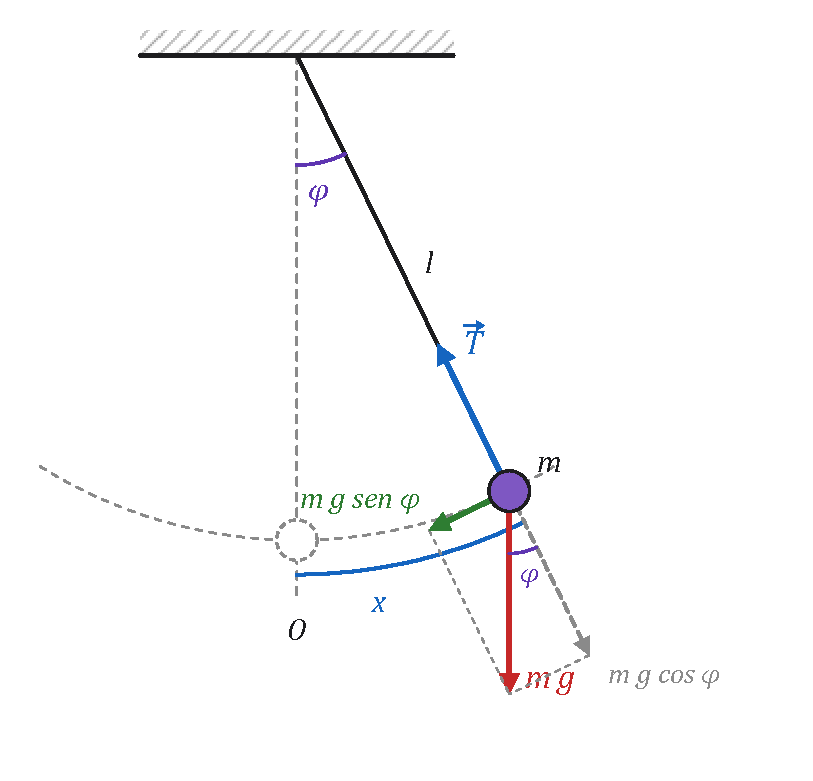
\includegraphics[width=0.5\linewidth]{images/UD1/pendulo}
    \caption{Fuerzas sobre un péndulo simple. La componente tangencial del peso, \(m g \sen\varphi\), lo devuelve hacia \(O\).}
    \label{fig:mas-pendulo}
\end{figure}

Esta fuerza no es exactamente proporcional al desplazamiento, así que en general el péndulo \emph{no} hace un m.a.s. Pero
para ángulos pequeños (menos de unos \ang{10}) se cumple \(\sen\varphi \approx \varphi\) (en radianes), y el arco recorrido es
\(x = l\,\varphi\). Entonces:
\begin{equation*}
    F \approx -\,m g\,\varphi = -\,\dfrac{m g}{l}\,x
\end{equation*}
que tiene la forma \(F = -k\,x\) con \(k = \dfrac{m g}{l}\). Igualando con \(k = m\omega^2\):
\begin{equation*}
    m\,\omega^2 = \dfrac{m g}{l} \;\Rightarrow\; \omega^2 = \dfrac{g}{l} \;\Rightarrow\; \dfrac{4\pi^2}{T^2} = \dfrac{g}{l}
\end{equation*}
\begin{centeredequation}
    \boxed{T = 2\pi\sqrt{\dfrac{l}{g}}} \label{eq:mas-periodo-pendulo}
\end{centeredequation}

\begin{remark}
    Para oscilaciones pequeñas, el período de un péndulo depende solo de su longitud y del valor de \(g\): \textbf{no depende
    de la masa ni de la amplitud} (isocronismo). Es proporcional a \(\sqrt l\) e inversamente proporcional a \(\sqrt g\), por
    eso un péndulo permite medir la gravedad (práctica~\ref{subsec:mas-practica-pendulo}).
\end{remark}

\begin{exercise}
    Comprueba con la calculadora la aproximación \(\sen\varphi \approx \varphi\) para \ang{2}, \ang{5}, \ang{10}, \ang{15} y
    \ang{20}. ¿Qué error relativo se comete en cada caso?
    \begin{solu}
        \textcolor{blue}{Pasamos cada ángulo a radianes y comparamos con su seno; error \(= (\varphi - \sen\varphi)/\sen\varphi\):}
        \begin{center}
            \begin{tabular}{@{}cccc@{}}
                \toprule
                \textbf{Ángulo} & \(\varphi\) (\unit{\radian}) & \(\sen\varphi\) & \textbf{Error} \\
                \midrule
                \ang{2} & \num{0.0349} & \num{0.0349} & \qty{0.02}{\percent} \\[3pt]
                \ang{5} & \num{0.0873} & \num{0.0872} & \qty{0.13}{\percent} \\[3pt]
                \ang{10} & \num{0.1745} & \num{0.1736} & \qty{0.51}{\percent} \\[3pt]
                \ang{15} & \num{0.2618} & \num{0.2588} & \qty{1.15}{\percent} \\[3pt]
                \ang{20} & \num{0.3491} & \num{0.3420} & \qty{2.06}{\percent} \\
                \bottomrule
            \end{tabular}
        \end{center}
        \textcolor{red}{Hasta \ang{10} el error no llega al \qty{0.5}{\percent}: la aproximación es muy buena.}
    \end{solu}
\end{exercise}

\begin{exercise}
    Un péndulo simple es cuatro veces más largo que otro. ¿Qué relación hay entre sus períodos?
    \begin{solu}
        \[ \dfrac{T_1}{T_2} = \dfrac{2\pi\sqrt{l_1/g}}{2\pi\sqrt{l_2/g}} = \sqrt{\dfrac{l_1}{l_2}} = \sqrt 4 = 2 \;\Rightarrow\; \textcolor{red}{T_1 = 2\,T_2} \]
    \end{solu}
\end{exercise}

\begin{exercise}
    Un reloj de péndulo bate segundos (\(T = \qty{2}{\second}\)) en un lugar donde \(g = \qty{9.81}{\m\per\second\squared}\).
    Lo llevamos a otro lugar donde \(g = \qty{9.78}{\m\per\second\squared}\).
    \begin{enumerate}[label=\letraminuscula]
        \item ¿Cuál será su nuevo período?
        \item ¿Cuánto se atrasará o adelantará en un día?
    \end{enumerate}
    \begin{solu}
        \begin{enumerate}[label=\letraminuscula]
            \item \textcolor{blue}{La longitud no cambia: \(\dfrac{T'}{T} = \sqrt{\dfrac{g}{g'}}\).}
            \(T' = 2\sqrt{\dfrac{9{,}81}{9{,}78}} = \textcolor{red}{\qty{2.0031}{\second}}\).
            \item \textcolor{blue}{En un día (\qty{86400}{\second}) da \(86400/2{,}0031 = \num{43134}\) oscilaciones, y el reloj cuenta
            \qty{2}{\second} por cada una: marca \(\qty{86268}{\second}\).}
            \textcolor{red}{Se atrasa unos \qty{132}{\second} (algo más de 2 minutos) al día.}
        \end{enumerate}
    \end{solu}
\end{exercise}

\section{Energía del movimiento armónico simple}\label{sec:mas-energia}

Un oscilador tiene dos tipos de energía: \textbf{cinética}, por su velocidad, y \textbf{potencial elástica}, asociada a la
fuerza recuperadora.

\paragraph{Energía cinética.} Con \(v = A\omega\cos(\omega t + \varphi_0)\) y \(k = m\omega^2\):
\begin{equation*}
    E_c = \dfrac{1}{2} m v^2 = \dfrac{1}{2} m A^2\omega^2\cos^2(\omega t + \varphi_0) = \dfrac{1}{2} k A^2\left[1 - \sen^2(\omega t + \varphi_0)\right]
    \;\Rightarrow\; \boxed{E_c = \dfrac{1}{2} k\,(A^2 - y^2)}
\end{equation*}
Es máxima en el centro (\(y = 0\)) y nula en los extremos (\(y = \pm A\)).

\paragraph{Energía potencial elástica.} La fuerza recuperadora es conservativa; su trabajo es igual a menos la variación de
energía potencial. Tomando \(E_p = 0\) en \(y = 0\):
\begin{equation*}
    W_{F_e} = -\Delta E_p \;\Rightarrow\; E_p = -\int_0^y (-k\,y)\,dy = k\left[\dfrac{y^2}{2}\right]_0^y \;\Rightarrow\; \boxed{E_p = \dfrac{1}{2} k\,y^2}
\end{equation*}
Es nula en el centro y máxima en los extremos.

\paragraph{Energía mecánica.} Sumando ambas:
\begin{centeredequation}
    E_m = E_c + E_p = \dfrac{1}{2}k(A^2 - y^2) + \dfrac{1}{2}k y^2 = \boxed{\dfrac{1}{2} k A^2} = \dfrac{1}{2} m\omega^2 A^2 = 2\pi^2 m \nu^2 A^2 \label{eq:mas-energia}
\end{centeredequation}

\begin{remark}
    Si no hay rozamiento, la energía mecánica de un oscilador \textbf{se conserva} y es proporcional al cuadrado de la
    amplitud (y al cuadrado de la frecuencia). Durante la oscilación la energía pasa continuamente de potencial (extremos) a
    cinética (centro) y al revés (figura~\ref{fig:mas-energia}).
\end{remark}

\begin{figure}[H]
    \centering
    \begin{tikzpicture}
        \begin{axis}[fisica, width=0.62\linewidth, height=5.6cm, xmin=-1.25, xmax=1.3, ymin=0, ymax=1.3,
            xlabel={\(y\)}, ylabel={\(E\)}, xtick={-1,1}, xticklabels={\(-A\),\(A\)},
            ytick={1}, yticklabels={\(\frac{1}{2}kA^2\)}, legend style={font=\small, at={(1.02,0.62)}, anchor=west, draw=none}]
            \addplot[domain=-1:1, very thick, red] {x^2};
            \addlegendentry{\(E_p = \frac{1}{2}k y^2\)}
            \addplot[domain=-1:1, very thick, blue] {1-x^2};
            \addlegendentry{\(E_c = \frac{1}{2}k(A^2-y^2)\)}
            \addplot[domain=-1:1, very thick, ocre] {1};
            \addlegendentry{\(E_m\)}
            \draw[dashed, gray] (axis cs:0.55,0) -- (axis cs:0.55,1);
            \draw[<->, red, thick] (axis cs:0.62,0) -- node[right, font=\scriptsize]{\(E_p\)} (axis cs:0.62,0.3025);
            \draw[<->, blue, thick] (axis cs:0.62,0.3025) -- node[right, font=\scriptsize]{\(E_c\)} (axis cs:0.62,1);
        \end{axis}
    \end{tikzpicture}
    \caption{Energías de un oscilador en función de la elongación. En cualquier posición \(E_c + E_p = E_m\).}
    \label{fig:mas-energia}
\end{figure}

\begin{exercise}
    Un cuerpo de \qty{0.5}{\kg} unido a un muelle de \qty{200}{\newton\per\m} oscila con una amplitud de \qty{10}{\cm}.
    Calcula su energía mecánica y, cuando está a \qty{5}{\cm} del equilibrio, sus energías potencial y cinética y su velocidad.
    \begin{solu}
        \textcolor{blue}{\(E_m = \frac{1}{2}kA^2 = \frac{1}{2}\cdot 200\cdot 0{,}1^2\)} \(= \textcolor{red}{\qty{1}{\joule}}\).

        \textcolor{blue}{En \(y = \qty{0.05}{\m}\):} \(E_p = \frac{1}{2}\cdot 200\cdot 0{,}05^2 = \textcolor{red}{\qty{0.25}{\joule}}\);
        \(E_c = E_m - E_p = \textcolor{red}{\qty{0.75}{\joule}}\).

        \(v = \sqrt{\dfrac{2E_c}{m}} = \sqrt{\dfrac{2\cdot 0{,}75}{0{,}5}} = \textcolor{red}{\qty{1.73}{\m\per\second}}\).
        \textcolor{blue}{(A mitad de la amplitud solo una cuarta parte de la energía es potencial.)}
    \end{solu}
\end{exercise}

\section{Resumen de fórmulas}\label{sec:mas-resumen}

\begin{table}[H]
    \centering
    \caption{Fórmulas principales del movimiento armónico simple}
    \vspace{-5pt}
    \begin{tabular}{@{}lll@{}}
        \toprule
        \textbf{Magnitud} & \textbf{Expresión} & \textbf{Valor máximo} \\
        \midrule
        Elongación & \(y = A\sen(\omega t + \varphi_0)\) & \(A\) \\[3pt]
        Velocidad & \(v = A\omega\cos(\omega t + \varphi_0) = \pm\,\omega\sqrt{A^2 - y^2}\) & \(A\omega\) (en el centro) \\[3pt]
        Aceleración & \(a = -A\omega^2\sen(\omega t + \varphi_0) = -\omega^2 y\) & \(A\omega^2\) (en los extremos) \\[3pt]
        Fuerza recuperadora & \(F = -k\,y\), \quad \(k = m\omega^2\) & \(kA\) \\[3pt]
        Período (muelle) & \(T = 2\pi\sqrt{m/k}\) & --- \\[3pt]
        Período (péndulo) & \(T = 2\pi\sqrt{l/g}\) \quad (ángulos pequeños) & --- \\[3pt]
        Energías & \(E_c = \frac{1}{2}k(A^2 - y^2)\), \quad \(E_p = \frac{1}{2}k y^2\) & \(E_m = \frac{1}{2}kA^2\) \\
        \bottomrule
    \end{tabular}
    \label{tab:mas-resumen}
\end{table}

\section{Prácticas de laboratorio}\label{sec:mas-practicas}

\subsection{Práctica 1: el oscilador armónico}\label{subsec:mas-practica-muelle}

\noindent\begin{minipage}[t]{0.64\linewidth}
\textbf{Objetivo.} Estudiar cómo depende el período de un muelle de la masa que cuelga de él y calcular su constante elástica.

\textbf{Material.} Soporte con varilla y pinza, muelle, portapesas, pesas de distintas masas, regla y cronómetro.

\textbf{Procedimiento.}
\begin{enumerate}[label=\numberballmDarkTeal]
    \item Monta el muelle en el soporte (figura~\ref{fig:mas-practica-muelle}) y cuelga el portapesas con una primera masa.
    \item Separa la masa un poco de su posición de equilibrio (unos \qty{2}{\cm}) y suéltala.
    \item Mide el tiempo de 10 oscilaciones completas. Repite la medida tres veces y calcula la media; el período es esa
    media dividida entre 10.
    \item Repite el proceso con al menos otras tres masas distintas y anota los datos en la tabla.
\end{enumerate}
\end{minipage}\hfill
\begin{minipage}[t]{0.32\linewidth}
    \vspace{0pt}
    \centering
    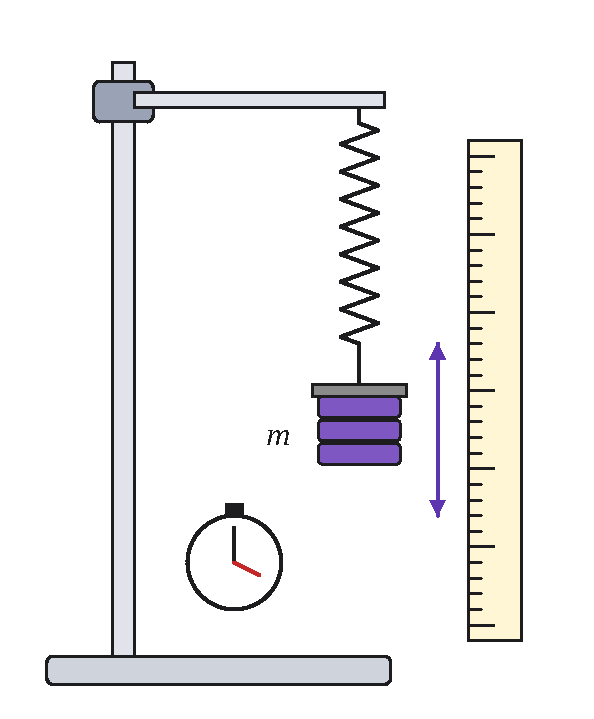
\includegraphics[width=0.9\linewidth]{images/UD1/practica_muelle}
    \captionof{figure}{Montaje de la práctica.}
    \label{fig:mas-practica-muelle}
\end{minipage}

\begin{table}[H]
    \centering
    \caption{Datos de la práctica del oscilador}
    \vspace{-5pt}
    \begin{tabular}{@{}C{2.2cm}C{3.4cm}C{2.2cm}C{2.2cm}C{2.6cm}@{}}
        \toprule
        \textbf{\(m\) (\unit{\kg})} & \textbf{Tiempo de 10 oscilaciones (\unit{\second})} & \textbf{\(T\) (\unit{\second})} & \textbf{\(T^2\) (\unit{\second\squared})} & \textbf{\(k\) (\unit{\newton\per\m})} \\
        \midrule
        \rule{0pt}{18pt} & & & & \\ \midrule[0.3pt]
        \rule{0pt}{18pt} & & & & \\ \midrule[0.3pt]
        \rule{0pt}{18pt} & & & & \\ \midrule[0.3pt]
        \rule{0pt}{18pt} & & & & \\
        \bottomrule
    \end{tabular}
    \label{tab:mas-practica-muelle}
\end{table}

\textbf{Cálculos.} De \(k = m\omega^2\) y \(\omega = 2\pi/T\) se obtiene:
\begin{equation*}
    T^2 = \dfrac{4\pi^2}{k}\,m
\end{equation*}
Con cada pareja \((m, T)\) calcula \(k = 4\pi^2 m / T^2\) y halla el valor medio.

\textbf{Método gráfico.} Representa \(T^2\) frente a \(m\). Los puntos deben quedar sobre una recta que pasa (casi) por el
origen, \(T^2 = b\,m\), cuya pendiente es \(b = 4\pi^2/k\). Traza la recta que mejor se ajuste y calcula \(k = 4\pi^2/b\).

\textbf{Cuestiones.}
\begin{enumerate}[label=\letraminuscula]
    \item ¿Por qué se mide el tiempo de 10 oscilaciones en lugar de una sola?
    \item Compara el valor de \(k\) obtenido con el cálculo directo y con la gráfica. ¿Cuál te parece más fiable y por qué?
    \item Cuelga una masa y mide el alargamiento \(\Delta l\). Calcula \(k = mg/\Delta l\) y compáralo con el obtenido.
\end{enumerate}

\subsection{Práctica 2: medida de \texorpdfstring{\(g\)}{g} con un péndulo simple}\label{subsec:mas-practica-pendulo}

\noindent\begin{minipage}[t]{0.64\linewidth}
\textbf{Objetivo.} Medir la aceleración de la gravedad con un péndulo simple y comprobar que, para oscilaciones pequeñas, su
período no depende de la amplitud ni de la masa.

\textbf{Material.} Soporte, doble nuez, varilla, hilo con una bola pequeña, regla graduada y cronómetro.

\textbf{Procedimiento.}
\begin{enumerate}[label=\numberballmDarkTeal]
    \item Monta el péndulo (figura~\ref{fig:mas-practica-pendulo}) y mide su longitud \(l\) desde el punto de suspensión
    hasta el centro de la bola.
    \item Sepáralo un ángulo pequeño (menos de \ang{10}) y suéltalo, cuidando de que oscile en un plano y no describa elipses.
    \item Mide el tiempo de 10 oscilaciones, repite la medida varias veces y calcula el período medio.
    \item Repite con otras longitudes. Para comprobar el isocronismo, repite una medida con otra amplitud (siempre pequeña)
    y con otra bola de distinta masa.
\end{enumerate}
\end{minipage}\hfill
\begin{minipage}[t]{0.32\linewidth}
    \vspace{0pt}
    \centering
    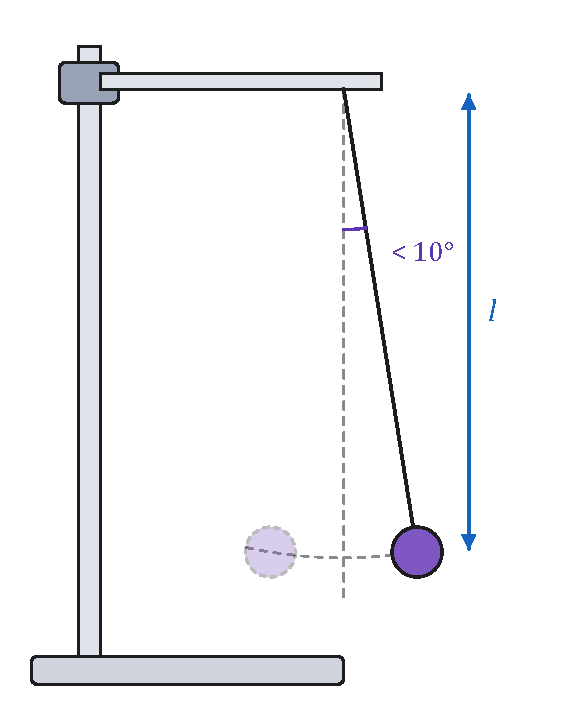
\includegraphics[width=0.9\linewidth]{images/UD1/practica_pendulo}
    \captionof{figure}{Montaje de la práctica.}
    \label{fig:mas-practica-pendulo}
\end{minipage}

\begin{table}[H]
    \centering
    \caption{Datos de la práctica del péndulo}
    \vspace{-5pt}
    \begin{tabular}{@{}C{2.6cm}C{3.6cm}C{2.4cm}C{2.4cm}C{2.4cm}@{}}
        \toprule
        \textbf{\(l\) (\unit{\m})} & \textbf{Tiempo de 10 oscilaciones (\unit{\second})} & \textbf{\(T\) (\unit{\second})} & \textbf{\(T^2\) (\unit{\second\squared})} & \textbf{\(g\) (\unit{\m\per\second\squared})} \\
        \midrule
        \rule{0pt}{18pt} & & & & \\ \midrule[0.3pt]
        \rule{0pt}{18pt} & & & & \\ \midrule[0.3pt]
        \rule{0pt}{18pt} & & & & \\ \midrule[0.3pt]
        \rule{0pt}{18pt} & & & & \\
        \bottomrule
    \end{tabular}
    \label{tab:mas-practica-pendulo}
\end{table}

\textbf{Cálculos.} De \(T = 2\pi\sqrt{l/g}\) se despeja \(g = \dfrac{4\pi^2 l}{T^2}\) para cada longitud.

\textbf{Método gráfico.} Representa \(T^2\) frente a \(l\): \(T^2 = \dfrac{4\pi^2}{g}\,l\) es una recta del tipo \(y = m x\)
con pendiente \(m = 4\pi^2/g\). Ajusta la recta y calcula \(g = 4\pi^2/m\).

\textbf{Cuestiones.}
\begin{enumerate}[label=\letraminuscula]
    \item ¿Has observado que el período cambie al usar otra bola o al soltar el péndulo desde otro ángulo pequeño?
    \item Calcula el error relativo de tu medida tomando como valor de referencia \(g = \qty{9.80}{\m\per\second\squared}\).
    \item ¿Qué ocurriría con el período si soltaras el péndulo desde \ang{45}? Justifícalo con la aproximación \(\sen\varphi \approx \varphi\).
\end{enumerate}
